%---------------------
% START OF PREAMBLE - do not delete!
%---------------------
\documentclass[12pt]{article}
\usepackage[pdftex]{graphicx}
\usepackage{amsmath}
\usepackage{verbatim}
\DeclareGraphicsRule{*}{mps}{*}{}

%==============================================================================
% Page layout
%==============================================================================

%------------------------------------------------------------------------------
%  Define the page dimensions.
%------------------------------------------------------------------------------
\setlength{\hoffset}{0.0in}
\setlength{\oddsidemargin}{0.0in}
\setlength{\evensidemargin}{0.0in}
\setlength{\textwidth}{6.75in}

\setlength{\voffset}{0in}
\setlength{\topmargin}{-.6in}
\setlength{\headheight}{12pt}
\setlength{\headsep}{12pt}
\setlength{\textheight}{9.5in}
\renewcommand{\baselinestretch}{1.0}
\renewcommand{\labelitemi}{-}

% writing the section number and the subsection number together
% and also the subsubsection in the form of 1.a
\renewcommand\thesubsection{\arabic{section}.\alph{subsection}}
\renewcommand\thesection{Problem \arabic{section}}
%------------------------------------------------------------------------------

%---------------------
% END OF PREAMBLE - do not delete!
%---------------------

\begin{document}

%---------------------
% make the title
%---------------------
\title{Homework 4}
\author{Masoud Akbarzadeh}
\date{\today}

\maketitle
% make these as info on top of the page
\begin{center}
    {\bf Estimated time to Completion}: {8 hours} \\
    {\bf Maximum Allocated Time}: {12 hours} \\
    {\bf Actual Time to Completion}: {12 hours} \\
    {\bf Collaborators}: {Nari, Juan, Amel, Brandon, Jennifer, Kat,Jesse, Delian} \\

\end{center}
%\newpage
%---------------------

%---------------------
% begin main text
%---------------------
\section{}\label{sec:problem-1}
\subsection{}\label{subsec:problem-1-a}

For computing the power spectrum of the time series, I used the 256 chunk size and 50\% overlap.

\begin{figure}
\begin{center}
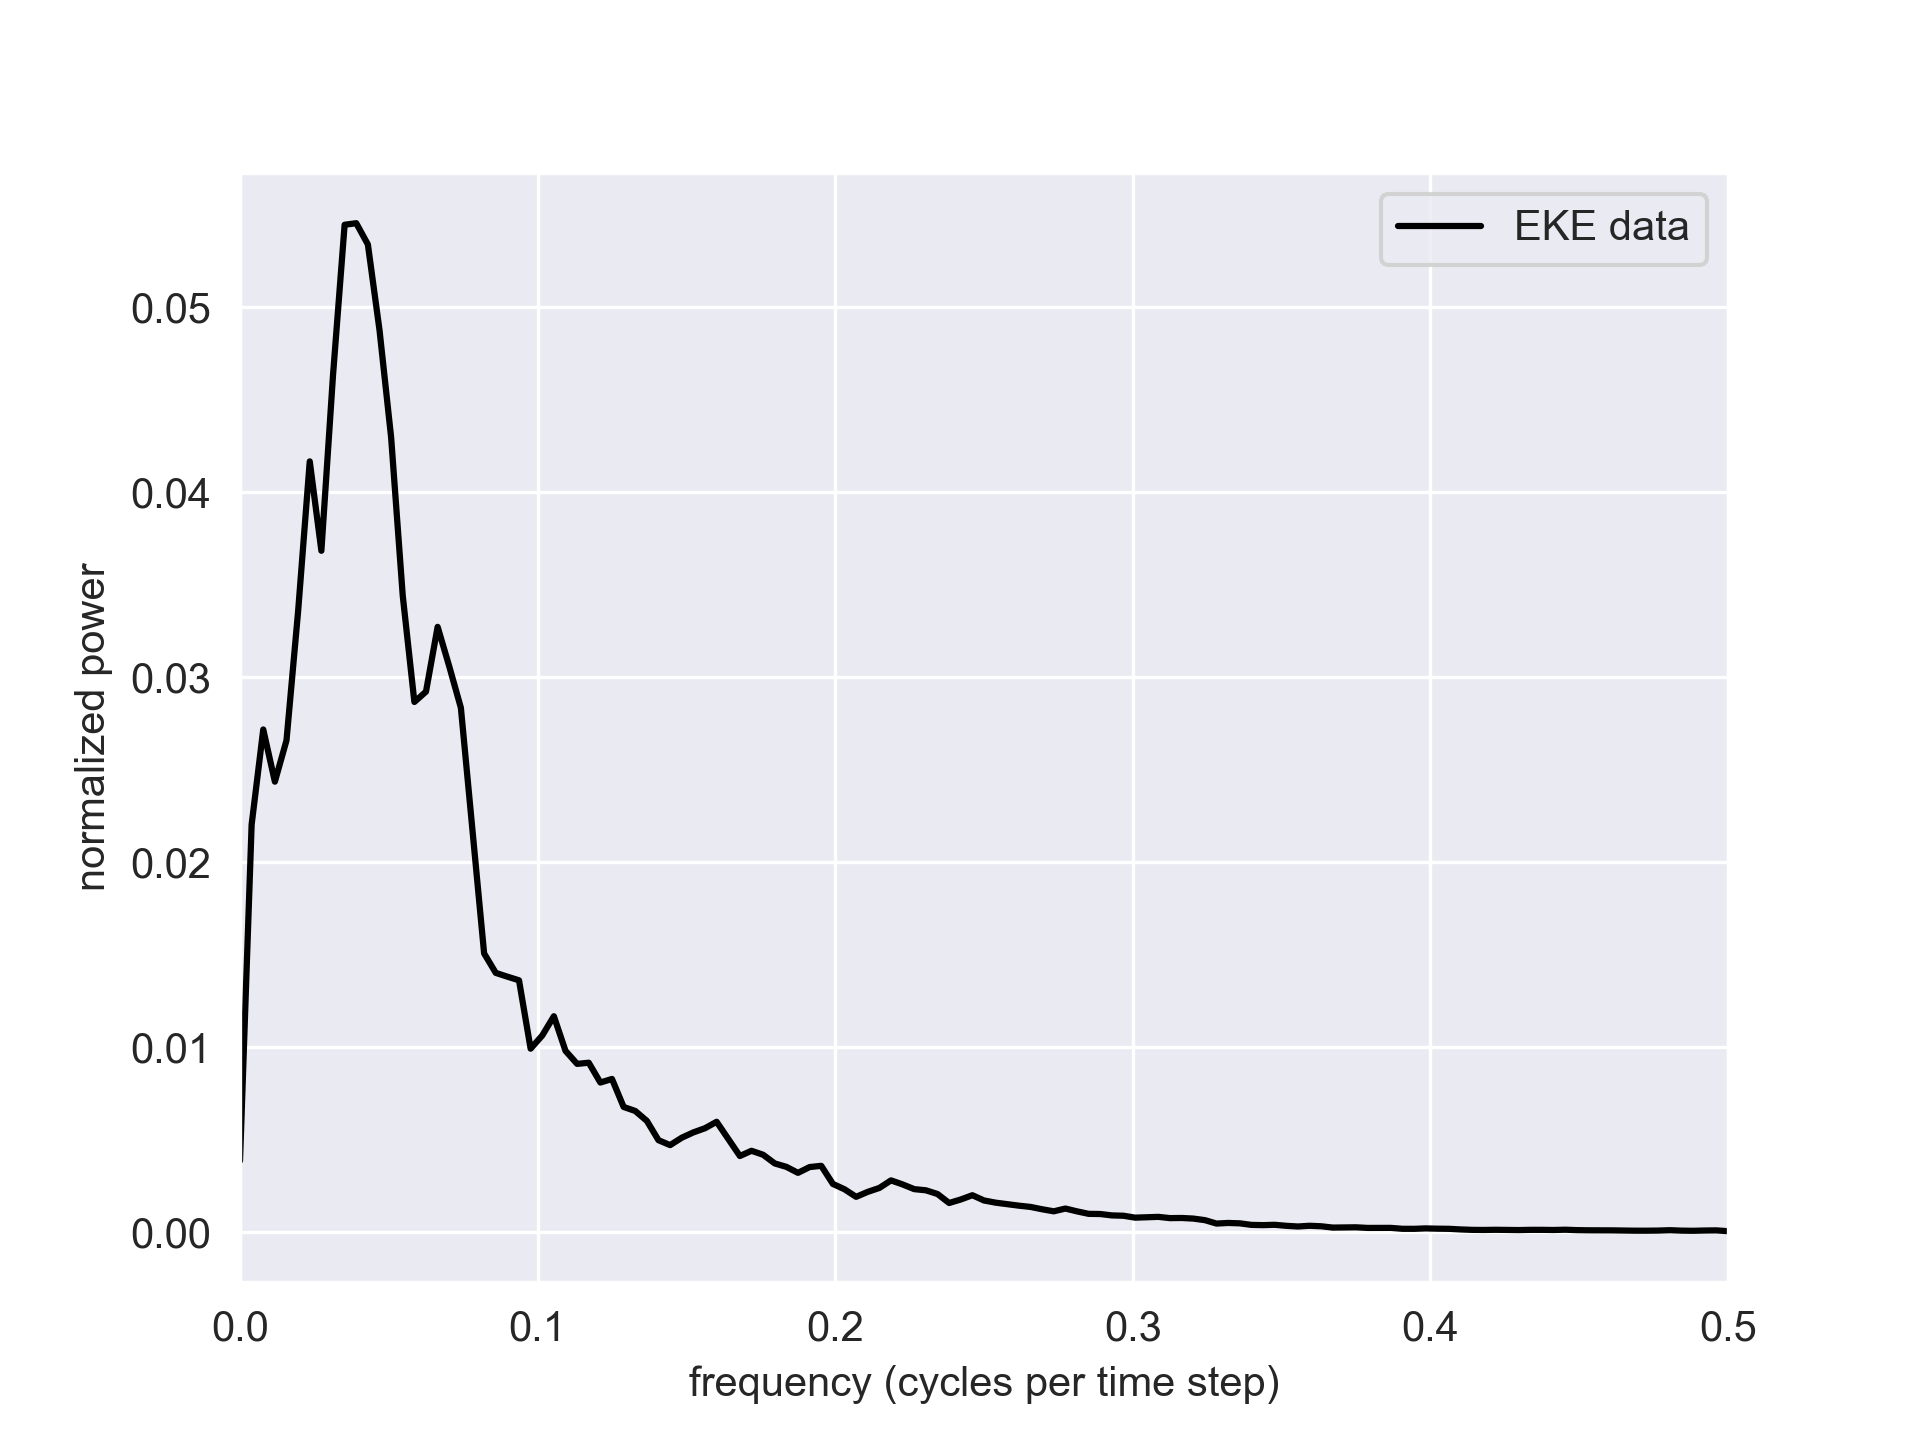
\includegraphics[width=6in]{hw4_pr1_1_power_spectrum_data.png}
\caption{Problem 1 - Plot of normalized power spectrum of EKE time series as a function of frequency}{\label{fig:problem-1-a}}
\end{center}
\end{figure}

\subsection{}\label{subsec:problem-1-b}
The significance of the spectral peaks was calculated using the red-noise null-hypothesis.
There are two distinct peaks at around 0.45 and 0.7 which are significant at the 99\% confidence level.

\begin{figure}
\begin{center}
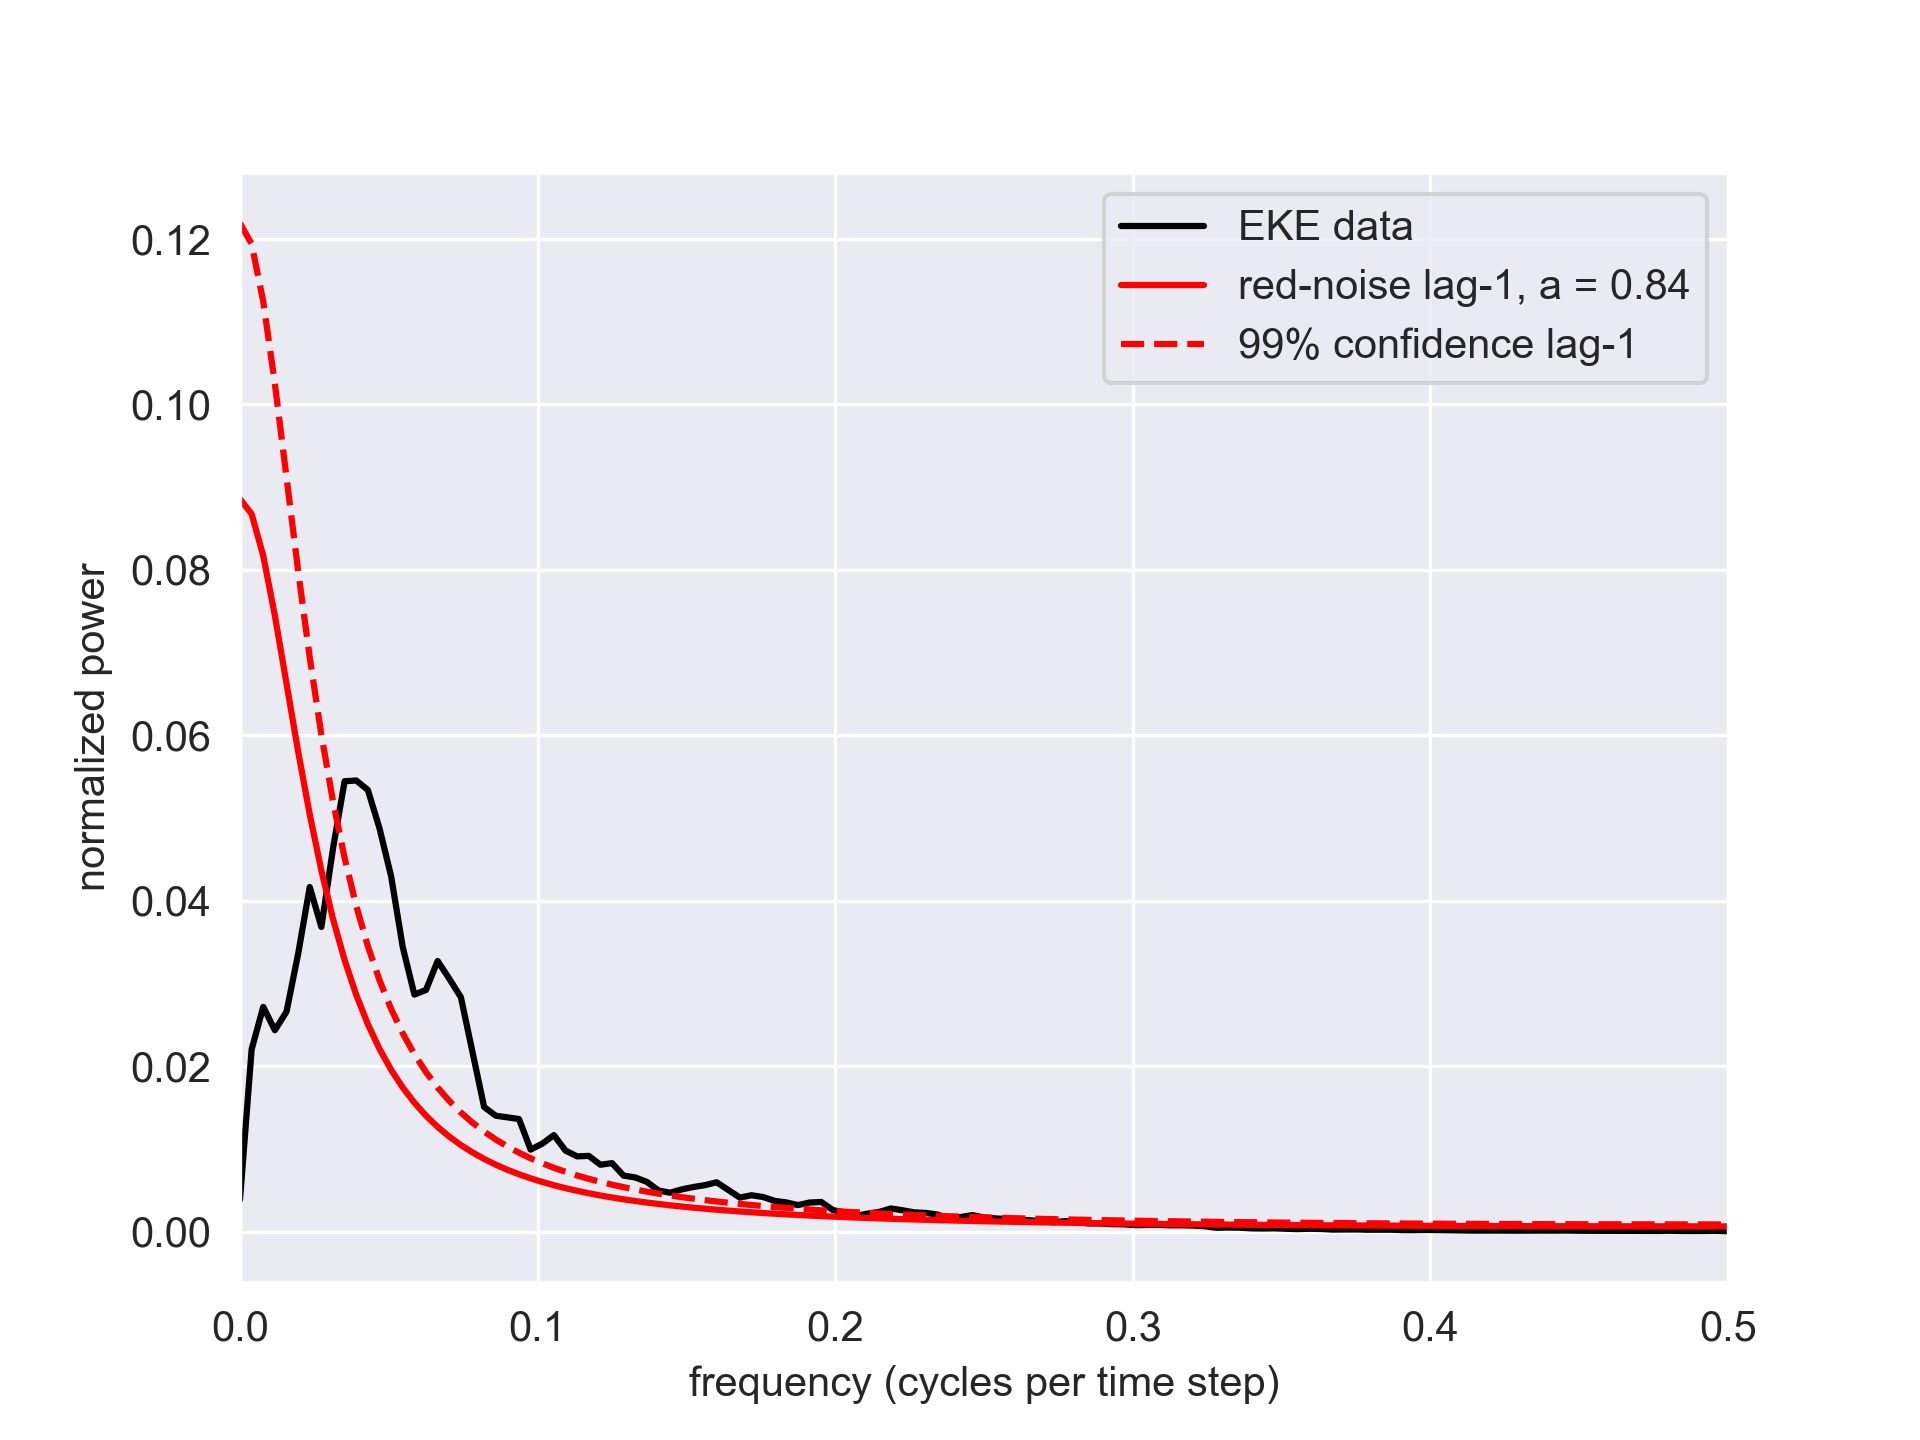
\includegraphics[width=6in]{hw4_pr1_2_power_spectrum_red_noise.png}
\caption{Problem 1 - Plot of normalized power spectrum and red-noise null-hypothesis as a function of frequency}{\label{fig:problem-1-a}}
\end{center}
\end{figure}

\subsection{}\label{subsec:problem-1-c}
The lag-1 autocorrelation and the e-folding time of the autocorrelation were computed and plotted.
Their values are considerably different in this example.
In this case the lag-1 autocorrelation is 0.84 and the e-folding autocorrelation is 0.72.
The reason for this difference might because the autocorrelation function may not decay at a constant exponential rate, which means the e-folding time, which assumes an exponential decay, might not capture the true decay behavior of the autocorrelation function
On the other hand, the rate of decay of the autocorrelation function changes dramatically after the first lag, which means the lag-1 autocorrelation is not perfect in capturing of the true decay behavior of the autocorrelation function.

\begin{figure}
\begin{center}
\includegraphics[width=6in]{hw4_pr1_0_autocorrelation.png}
\caption{Problem 1 - Plot of autocorrelation vs lag for EKE time series}{\label{fig:problem-1-a}}
\end{center}
\end{figure}

\begin{figure}
\begin{center}
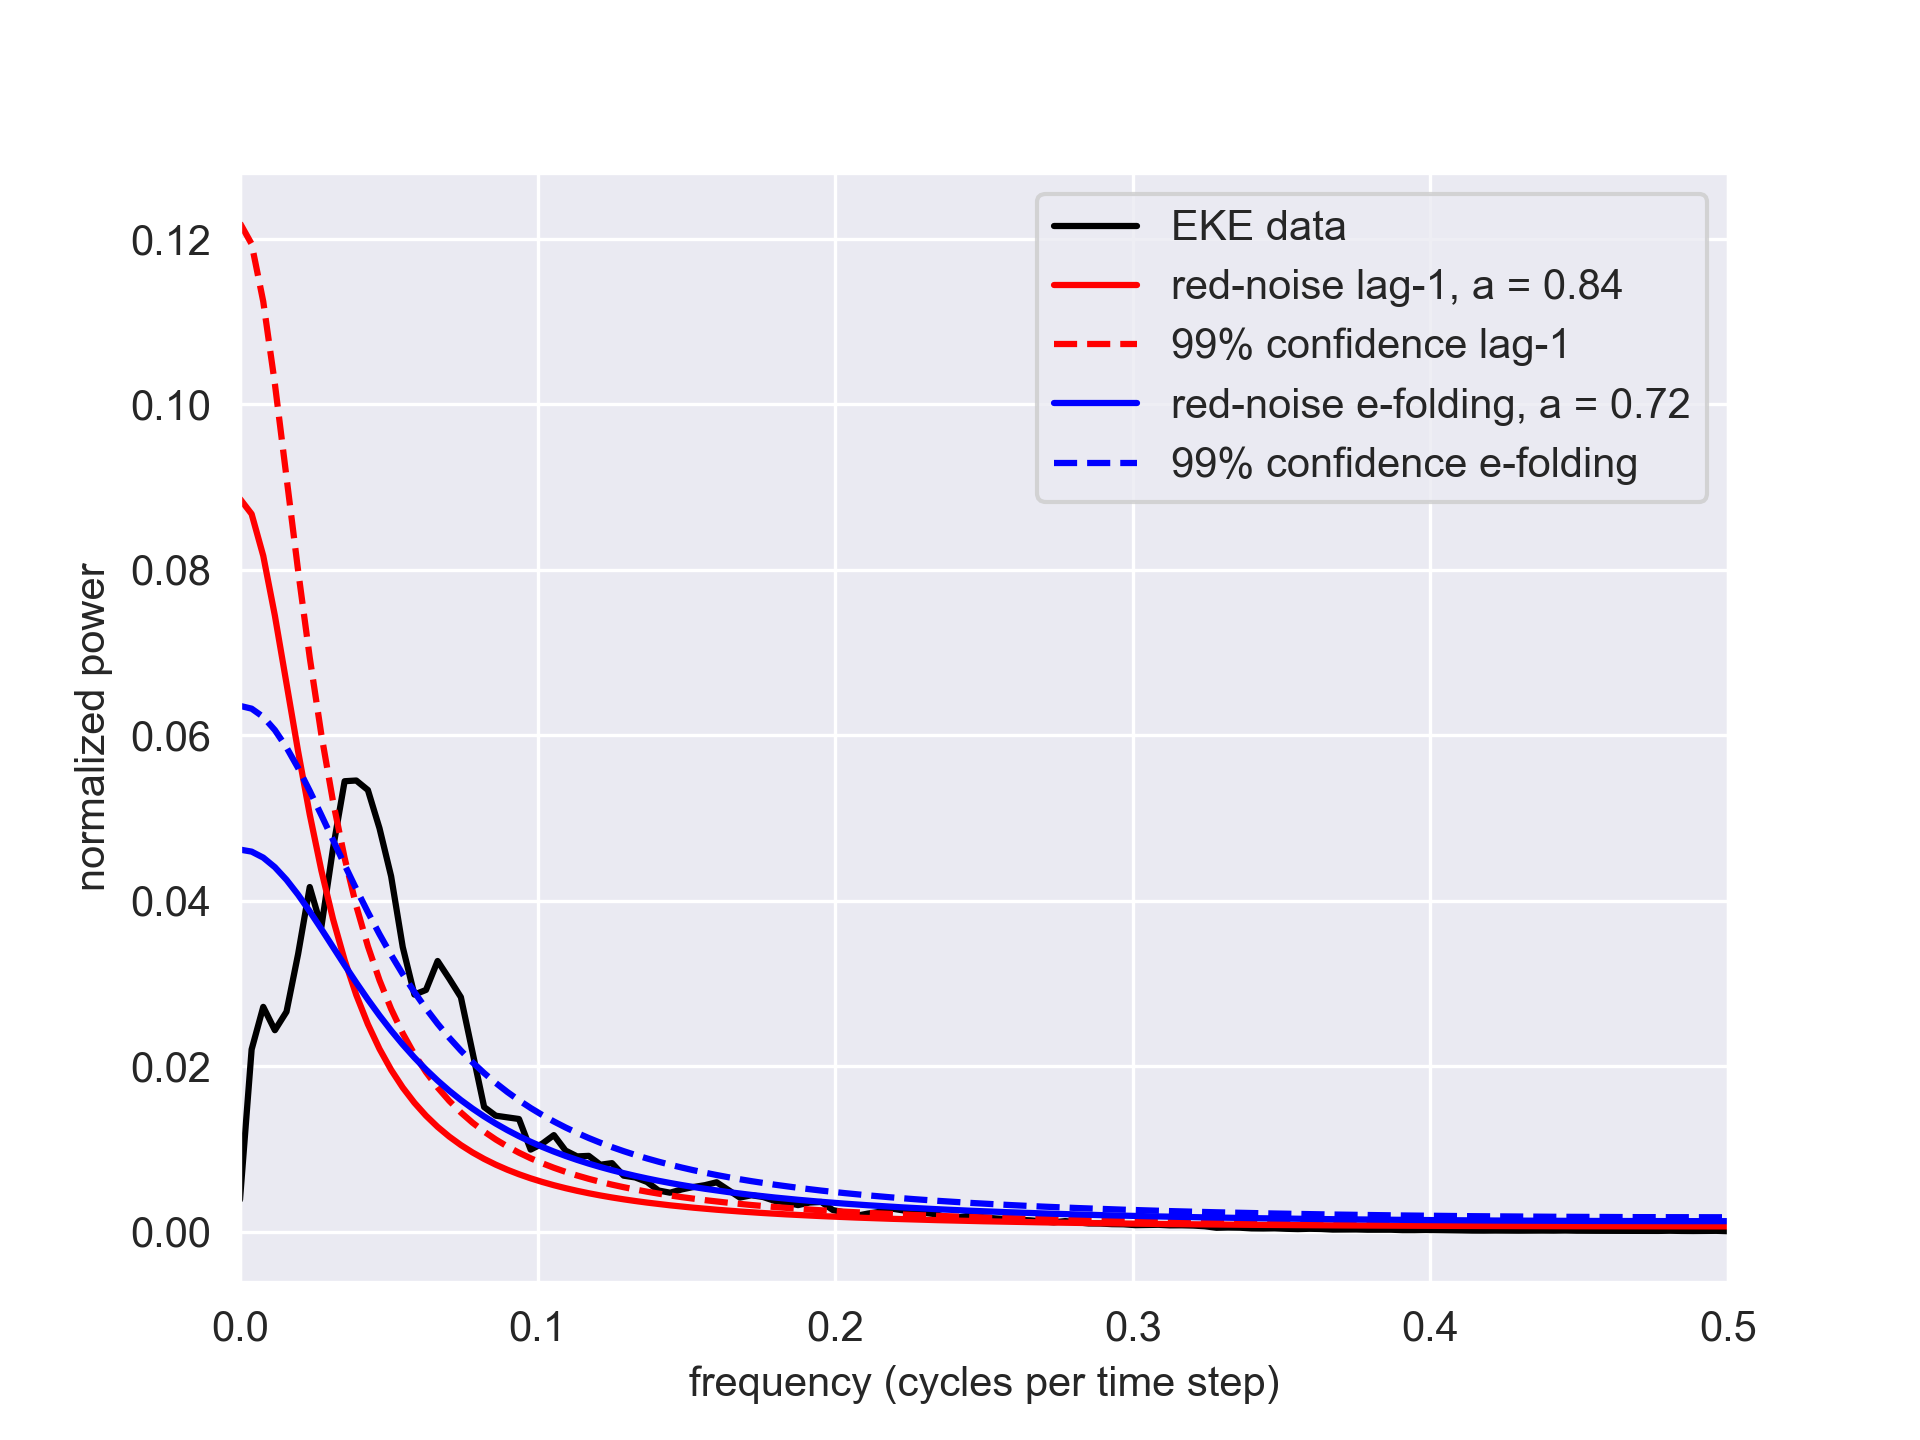
\includegraphics[width=6in]{hw4_pr1_3_power_spectrum_e_folding.png}
\caption{Problem 1 - Plot of normalized power spectrum and red-noise null-hypothesis based on lag-1 autocorrelation and e-folding time of autocoreealtion as a function of frequency}{\label{fig:problem-1-a}}
\end{center}
\end{figure}


\subsection{}\label{subsec:problem-1-d}
Using eaiher the lag-1 autocorrelation or the e-folding time of the autocorrelation, the power spectrum of the time series was compared to the red-noise null-hypothesis and plotted.
The most significant peak when comparing the power spectrum of the time series to the red-noise null-hypothesis is at the frequency of 0.045 and 0.07 Both of these peaks are significant at the 99\% confidence level if we use either the lag-1 autocorrelation or the e-folding time of the autocorrelation.
Since the time step is 1 day, these peaks are representative of phenomena that have 22 and 14 days time scales.



%new page
\newpage
\section{}\label{sec:problem-2}
The PM2.5 concentration in one of the stations in the city of Beijing was used as the time series for this problem.
The time series was divided into 256 chunks with 50\% overlap.
Because my data had more than 50,000 data points I had a range of options.
I used 256 samples chunk as it gives a suitable degree of freedom and also considers around 10 days chunks.
The power spectrum of the time series was computed and plotted.
Also, the degree of freedom for this analysis was computed as 198.
\\
The lag-1 autocorrelation and the e-folding time of the autocorrelation were also computed and plotted.
Their values are very close to each other in this case.
The lag-1 autocorrelation is 0.97 and the e-folding autocorrelation is 0.96. So I used the lag-1 autocorrelation for the red-noise null-hypothesis.
\\
The power spectrum of the time series was compared to the red-noise null-hypothesis and plotted.
The most significant peak when comparing the power spectrum of the time series to the red-noise null-hypothesis is at the frequency of 0.041.
Since the time step is 1 hour, the period of this peak is 24.4 hours.
This must be related to the daily cycle of the PM2.5 concentration in Beijing.
\begin{figure}
\begin{center}
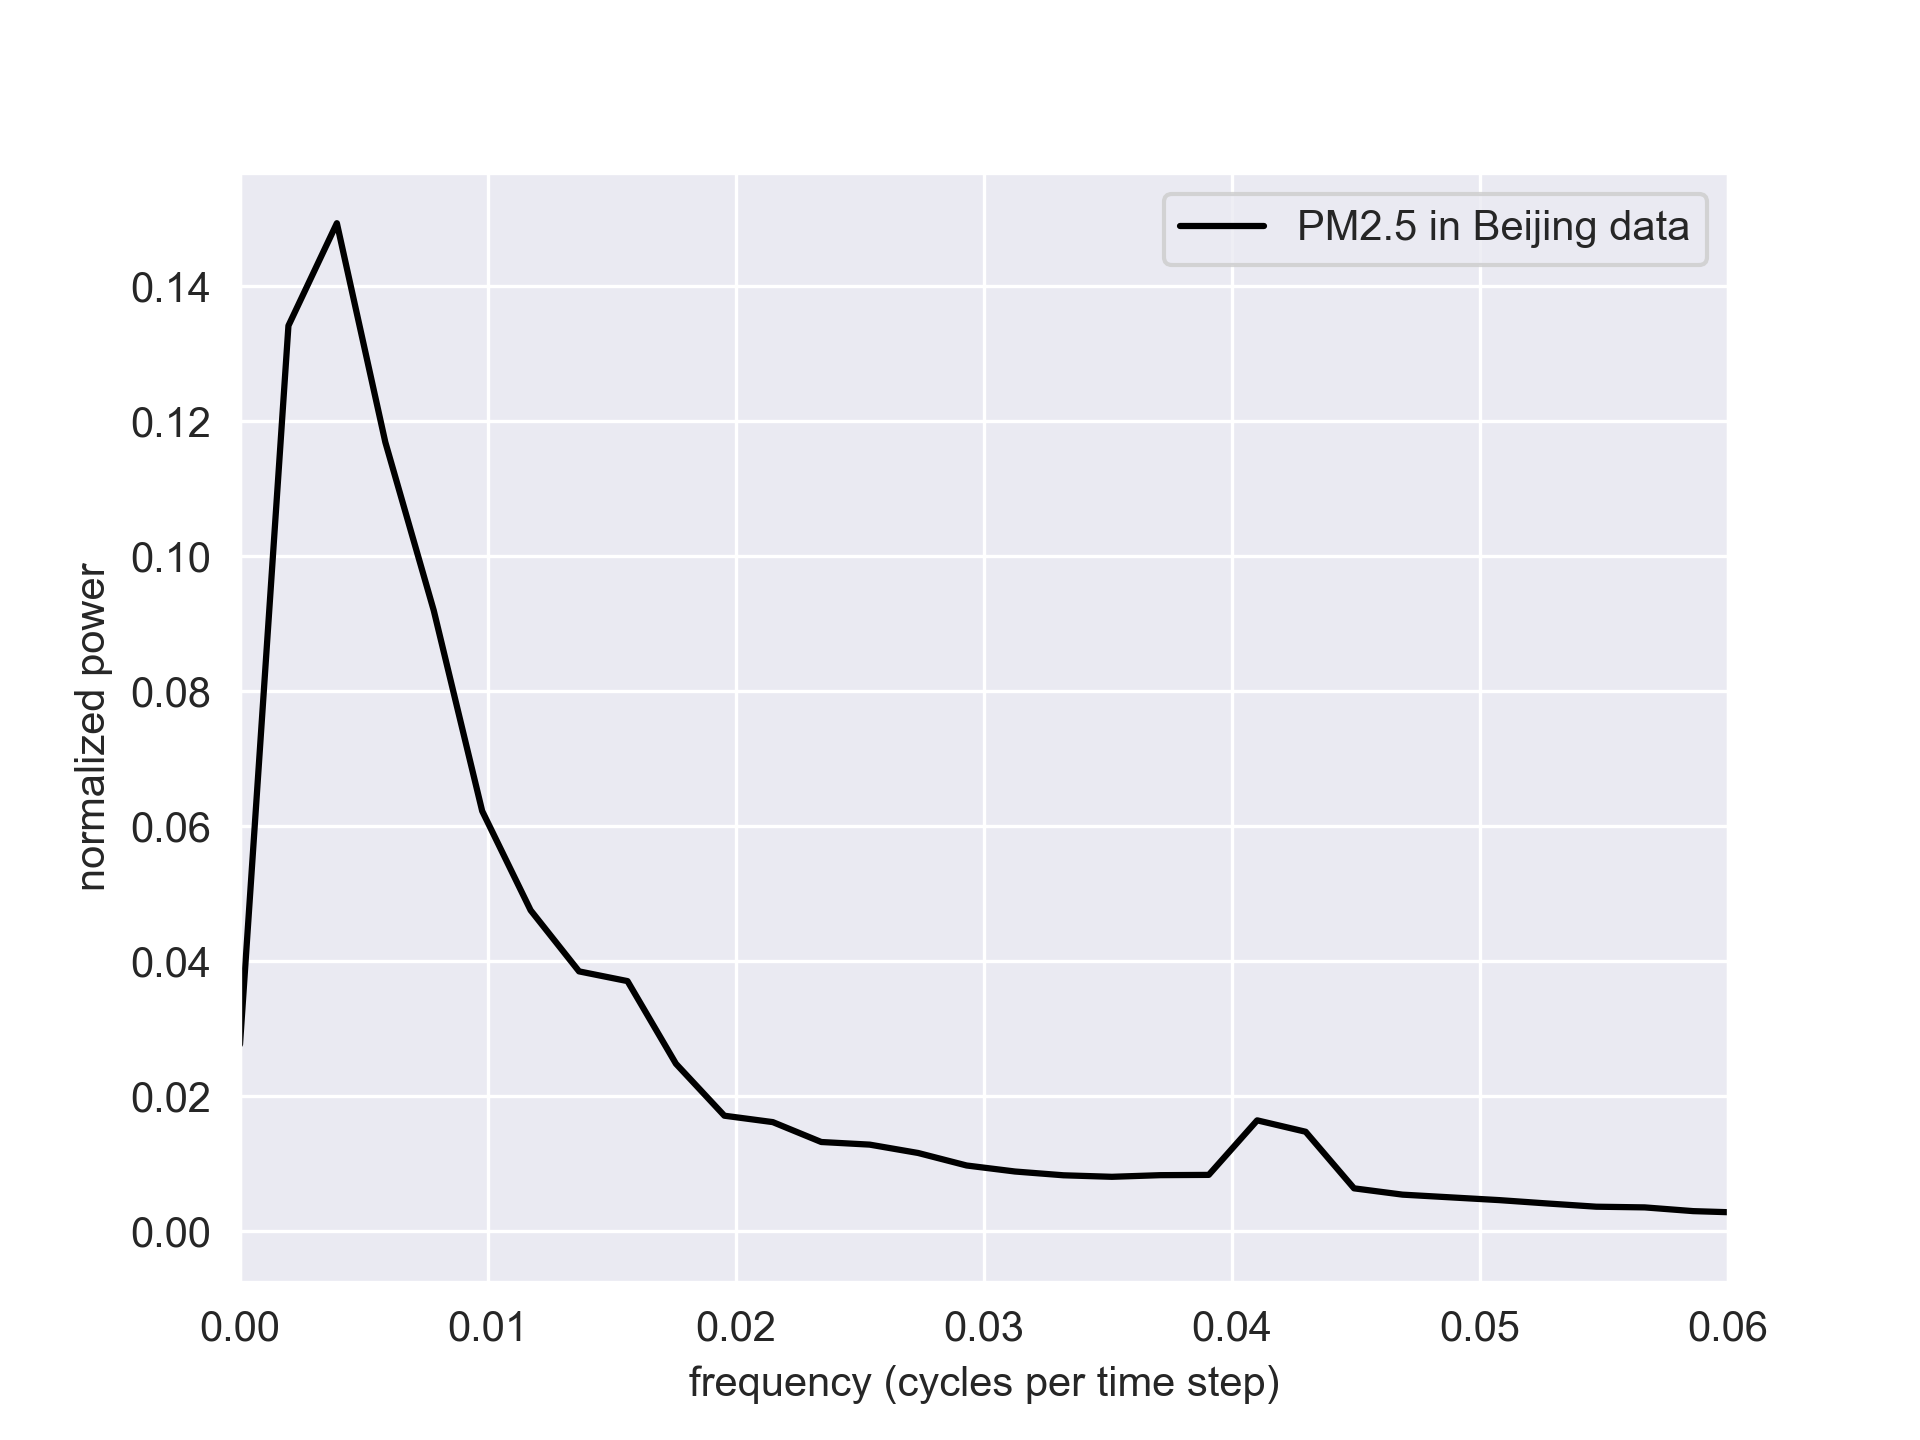
\includegraphics[width=6in]{hw4_pr2_1_power_spectrum_data.png}
\caption{Problem 2 - Plot of normalized power spectrum of PM2.5 time series as a function of frequency}{\label{fig:problem-1-a}}
\end{center}
\end{figure}

\begin{figure}
\begin{center}
\includegraphics[width=6in]{hw4_pr2_0_autocorrelation.png}
\caption{Problem 2 - Plot of autocorrelation vs lag for PM2.5 in Biejing}{\label{fig:problem-1-a}}
\end{center}
\end{figure}

\begin{figure}
\begin{center}
\includegraphics[width=6in]{hw4_pr2_4_power_spectrum_max_distance.png}
\caption{Problem 2 - Plot of normalized power spectrum of PM2.5 time series and red-noise null-hypothesis as a function of frequency}{\label{fig:problem-1-a}}
\end{center}
\end{figure}


\end{document}


